\documentclass{bsuir}
\usepackage{ulem}
\usepackage{makecell}
\usepackage{multirow}

\departmentlong{инженерной психологии и эргономики}
\worktitle{Практическая работа \textnumero1\\\textquote{Патентное исследование и
патентная информация}}
\titleleft{ Проверила:\\
    Фомин Д.А.\\
    ~
}
\titleright{
    Выполнил:\\
    Бородин А.Н.\\
    гр. 310901
}
\titlepageyear{2025}

\usepackage{pgfplots}
\usepackage{amsmath}
\usepackage{breqn}

\newlength{\tablewidth}
\setlength{\tablewidth}{\textwidth - \parindent}

\begin{document}

\maketitle
\mainmatter

\includepdf[pages=2-,angle=90]{work.pdf}

\end{document}
